\icode{N16-MCC-SI-L2-261023-002}
\nceeID[6]{2016全国\Rmnum{2}卷}{16}
小球\(P\)和\(Q\)用不可伸长的轻绳悬挂在天花板上，\(P\)球的质量大于\(Q\)球的质量，悬挂\(P\)球的绳比悬挂\(Q\)球的绳短。将两球拉起，使两绳均被水平拉直，如图所示。将两球由静止释放。在各自轨迹的最低点\paren[]

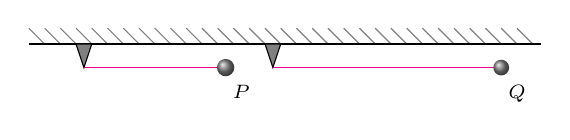
\begin{tikzpicture}[font=\scriptsize]
	\foreach \x in {-1.5,-1.3,...,4.8}
		\draw[gray] (\x,.2)--++(.2,-.2);
	\draw[thick](-1.5,0)--(5,0);
	\draw[fill=gray] (-.9,0)--(-.8,-.3)--(-.7,0)--(-.9,0);
	\draw[fill=gray] (1.5,0)--(1.6,-.3)--(1.7,0)--(1.5,0);
	\draw[magenta] (-.8,-.3)--(1,-.3) (1.6,-.3)--(4.5,-.3);
	\shade[ball color=gray] (1,-.3) circle(.11);
	\shade[ball color=gray] (4.5,-.3) circle(.1);
	\node at(1.2,-.4)[below]{\(P\)};
	\node at(4.7,-.4)[below]{\(Q\)};
\end{tikzpicture}
\begin{choices}
	\item \(P\)球的速度一定大于\(Q\)球的速度
	\item \(P\)球的动能一定小于\(Q\)球的动能
	\item \(P\)球所受绳的拉力一定大于\(Q\)球所受绳的拉力
	\item \(P\)球的向心加速度一定小于\(Q\)球的向心加速度
\end{choices}
\begin{answer}
	C\qquad 提示：最低点加速度相同，\(a_{\text{向}} = 2g\)
\end{answer}